%!TEX root=thesis.tex

\chapter{Radio Cross-identification}
\label{cha:passive-learning}
  % In this chapter I'll talk about a machine learning approach to the cross-identification problem (i.e. my pipeline).

  In this chapter, I develop a machine learning approach to the radio cross-identification problem. First, I will discuss different ways to train and use a classifier for the task, in particular framing the cross-identification problem as an object localisation problem. Then, I will discuss the available training data and how I chose to process it. Finally, I will present results against a dataset of expert labels, and compare these results to those found by other methods.

\section{Formalism}
\label{sec:cross-identification-formalism}
  
  \todo{Rewrite below into this section.}

  \todo{Explain why we're ignoring the radio part of this problem.}

  \subsection{Cross-identification as Object Localisation}
  \label{sec:object-localisation}

  \subsection{The Galaxy Classification Task}
  \label{sec:galaxy-classification-task}

% \section{Cross-identification as Binary Classification}
% \label{sec:framing-as-classification}
  
  When we look at the sky with radio telescopes, we see the radio emissions from
  the jets of AGNs. \todo{Add backlink.} Given an image of these radio
  emissions, we want to locate the host galaxy containing the associated AGN. In
  general, there may be multiple hosts associated with one radio object (such as
  in Figure \ref{fig:two-hosts}), but we make the assumption that there is only
  one. This is the same assumption made by Radio Galaxy Zoo \todo{cite:rgz-
  analysis-github(?)} and greatly simplifies the problem.

  \begin{figure}[!ht]
    \centering
    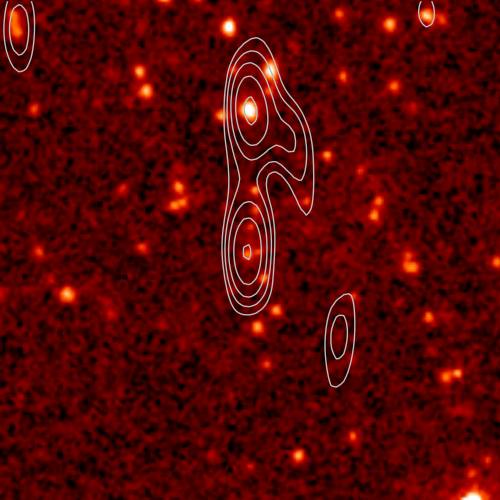
\includegraphics[width=0.5\textwidth]{images/CI0370C1_heatmap+contours.png}
    \caption{A radio object (ARG0003ra1) with two host galaxies. This radio
      object is actually two radio objects that have been incorrectly detected
      as one, and there is one host galaxy for each object.}
    \label{fig:two-hosts}
  \end{figure}

  We can interpret cross-identification as an object localisation problem. As
  input, we have an image of the radio sky, and we want to locate a host galaxy
  in this image. A common way to find an object in an image is by using a
  sliding window. A fixed-size image patch centred on each pixel is taken as a
  feature representation of that pixel. This is then used as input to a
  classification model which outputs a probability for each pixel, with higher
  probabilities corresponding to higher likelihood of the object being located
  at that pixel. The pixel with the highest rating is considered the location
  of the object. This approach can be improved by intelligently selecting
  candidate pixels and only testing these. For the cross-identification
  problem, we can use galaxy locations as candidate pixels, with galaxies found
  in infrared surveys such as WISE and SWIRE. Additionally, astronomical
  measurements such as flux are included in these surveys and these may be
  taken as additional features for each candidate pixel, giving more
  information to the classifier.

  This approach can be formalised as follows. Consider a set $\mathcal X$ of
  candidate host galaxies, and a radio object $r$ that we want to assign a
  host galaxy. Let $y : \mathcal X \to \{0, 1\}$ represent whether a given $x
  \in \mathcal X$ is the host galaxy associated with $r$. Under the assumption
  that a radio object has exactly one associated host galaxy, then there exists
  exactly one $x \in \mathcal X$ such that $y(x) = 1$, and for all other $x \in
  \mathcal X$, $y(x) = 0$. The cross-identification task then amounts to
  modelling $p(y(x) = 1 \mid x, r)$. Once this distribution is modelled, the
  host galaxy associated with $r$ is given by
  \begin{equation}
      \label{eq:cross-identification}
      \mbox{host}(r) = \underset{x}{\mbox{argmax}}\ p(y(x) = 1 \mid x, r).
  \end{equation}

  Ideally, $\mathcal X$ is the set of all galaxies. This is clearly
  intractable, so as an approximation we use a catalogue of infrared objects
  near the radio object of interest, taken from an infrared survey. We also
  make the assumption that the host galaxy is within $1'$ of the radio object
  --- while this doesn't hold in general, systems larger than $1'$ are rare and
  require human insight to discover \citep{banfield16}.

\section{Evaluating Performance Without Groundtruth}
\label{sec:norris-as-groundtruth}
  
  Our training labels for the classification task will come from the Radio
  Galaxy Zoo. While these labels can be aggregated in a number of ways to
  approximate the groundtruth (Section \ref{sec:rgz-crowd-labels}), these
  aggregates are \emph{not} the groundtruth and may contain high noise. This
  becomes a problem when we want to assess the performance of a trained
  classifier --- we want our classifier to be capable of finding the best
  approximation to the groundtruth, not to the noisy inputs, and evaluation
  should reflect that. We therefore cannot use aggregated crowd labels for
  evaluation.

  In general, though, we \emph{don't} have groundtruth for this problem, and
  while the groundtruth exists (a galaxy either has an AGN or does not), it is
  impossible for us to measure this accurately. Even expert catalogues, such as
  those provided by \citeauthor{norris06} (Section \ref{sec:norris}), are noisy
  --- \citep{norris06} estimate that their cross-identifications have a $9.02\%$
  false positive rate.

  To attempt to mitigate this problem, we chose a test set with as little noise
  as possible by combining the \citeauthor{fan15} catalogue (Section
  \ref{sec:fan}) with the \citeauthor{norris06} catalogue (Section
  \ref{sec:norris}) to find all galaxies for which the two catalogues agree.
  Test sets were drawn from only these galaxies. This does mean that the test
  instances will be ``easier'' than a test set drawn from the entire data set,
  but any tests performed against these test sets should be more reliable than
  would otherwise be the case.

\section{Feature Selection}
\label{sec:features}

  To train a machine learning method to solve the galaxy classification task,
  we must find a representation of galaxies in a feature space $\mathbb{R}^D$.
  In this section we describe and motivate our choice of galaxy features,
  extracted from both infrared and radio surveys.

  \subsection{Infrared Features}
  \label{sec:ir-features}

    As described in Section \ref{sec:cross-identification-formalism}, we need
    candidate host galaxies from an infrared catalogue. We have two choices here
    --- the SWIRE catalogue (Section \ref{sec:swire}) and the WISE catalogue
    (Section \ref{sec:wise}). SWIRE has higher resolution and sensitivity, and
    thus would give more accurate galaxies, but it does not cover the whole sky.
    WISE is lower resolution and less sensitive, but is the survey that will be
    used to cross-identify EMU (Section \ref{sec:emu}) sources when they are
    available. Here, we describe our choice of features for both.

    The WISE catalogue contains magnitude information for each object. There are
    four such magnitudes --- $w1$, $w2$, $w3$, and $w4$ --- each representing
    the amount of light emitted by the object in a different range of
    wavelengths.

    We chose to use all four magnitudes as features. Since the features are
    magnitudes, they are on a logarithmic scale, and we found that in practice
    classification performance improved when the magnitudes were converted to
    fluxes. We performed this conversion with the formula
    \[
      f = 10^{-0.4m}
    \]
    where $f$ is the flux and $m$ is the magnitude. This is the inverse of
    Equation \ref{eq:apparent-magnitude}, and gives the flux in arbitrary, but
    linear, units.

    \begin{figure}[!ht]
      \centering
      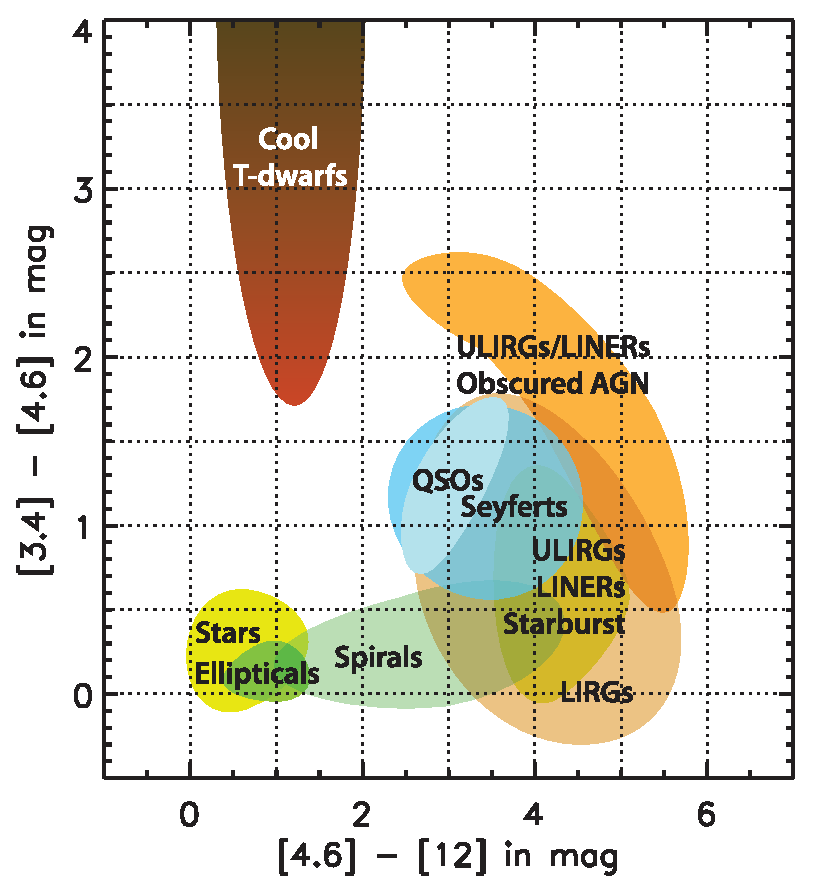
\includegraphics[width=0.5\textwidth]{images/wise_colour-colour}
      \caption{WISE colour-colour diagram showing the colours of various
        astronomical objects. The horizontal axis is $w2 - w3$ and the vertical
        axis is $w1 - w2$. Reproduced from \citep{wright10}.}
      \label{fig:wise-colour-colour}
    \end{figure}

    The ratios between infrared fluxes are indicators of physical galactic
    properties such as star formation and dust \todo{Find a source on this ---
    Probably the WISE paper wright10}. In practice, the $w1 - w2$ and $w2 - w3$
    ratios are most commonly used (such as in Figure
    \ref{fig:wise-colour-colour}), so we chose to use these ratios as features.
    Once again, we used a linear scale, computing the ratios using equation
    \ref{eq:magnitude-difference}.

    Also available were the unprocessed infrared images captured in the survey.
    Under the assumption that the large scale infrared structure of a galaxy is
    unchanged by an AGN, we chose to ignore the images themselves and focus on
    features obtained from the catalogue. This greatly simplified feature
    selection with minimal expected impact on the classification performance.
    Future work may investigate the effectiveness of features extracted from
    infrared images on classification performance, but this is out of the scope
    of this thesis.

    SWIRE also contains colour information, but unlike WISE, the information is
    in the form of fluxes instead of magnitudes. This means that the flux
    information in the catalogue can be used as features directly. The ratios
    can also be used --- $3.6\ \mu\text{Jy} / 4.5\ \mu\text{Jy}$ and $4.5\
    \mu\text{Jy} / 5.8\ \mu\text{Jy}$ are the SWIRE equivalents of $w1 - w2$ and
    $w2 - w3$. Since SWIRE is higher resolution than WISE, the
    infrared images may contain more useful information and thus be useful for
    features, but this was not explored in this thesis.

    % The SWIRE catalogue (Section \ref{sec:swire}) also contains colour
    % information for each contained object, but only fluxes rather than
    % magnitudes. \todo{Read the SWIRE colour-colour diagram and continue this.}

    % Both WISE and SWIRE catalogues contain the positions of each object. The
    % distance from each object to the centre of the closest radio object is
    % used as a feature representing that object. This noticeably improves
    % classification performance \todo{make an experiment showing this, and
    % probably also showing that the other features are good}.

  \subsection{Radio Features}
  \label{sec:image-features}

    While the infrared catalogues include measurements on individual galaxies,
    the ATLAS radio catalogue does not. This is because galaxies are not
    visible in radio, so while galaxies are directly represented in an infrared
    catalogue they are not in a radio catalogue. Galactic features must thus be
    extracted from the radio images directly. We chose to use a convolutional
    neural network, as described in Section \ref{sec:image-features}.

    \subsubsection{Building a Model for Feature Extraction}
    \label{sec:feature-extraction-model}

      We chose to use a convolutional neural network (CNN) with three
      convolutional and max pooling layers, shown in Figure \ref{fig:radio-cnn}.
      This resulted in an 128-dimensional feature vector. For training this
      network, we added a 64-dimensional dense layer mapping to a 1-dimensional
      output. 10\% of ATLAS objects were selected at random and reserved for
      training the CNN, to ensure later testing data would not overlap the
      training set. The entire network was then trained to match the consensus
      Radio Galaxy Zoo labels of the galaxies nearest the reserved training set.

      \begin{figure}[!ht]
         \centering
         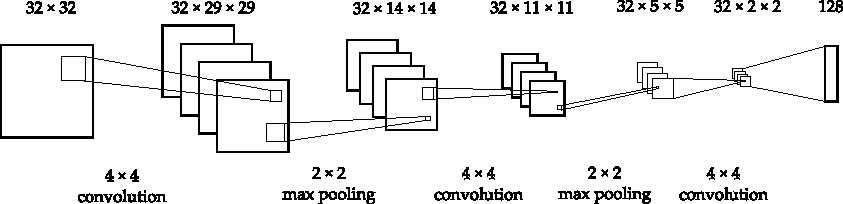
\includegraphics[width=\textwidth]{images/cnn_new.pdf}
         \caption{Convolutional neural network for radio feature extraction.}
         \label{fig:radio-cnn}
       \end{figure}

      A better approach would be to use a convolutional autoencoder, which would
      allow training on all the radio data, and data with no labels at all, but
      this was computationally infeasible for this project.

      An example of the neural network applied to a radio image is shown in
      Figure \ref{fig:rgz-cnn}.

      \begin{figure}[!ht]
        \centering
        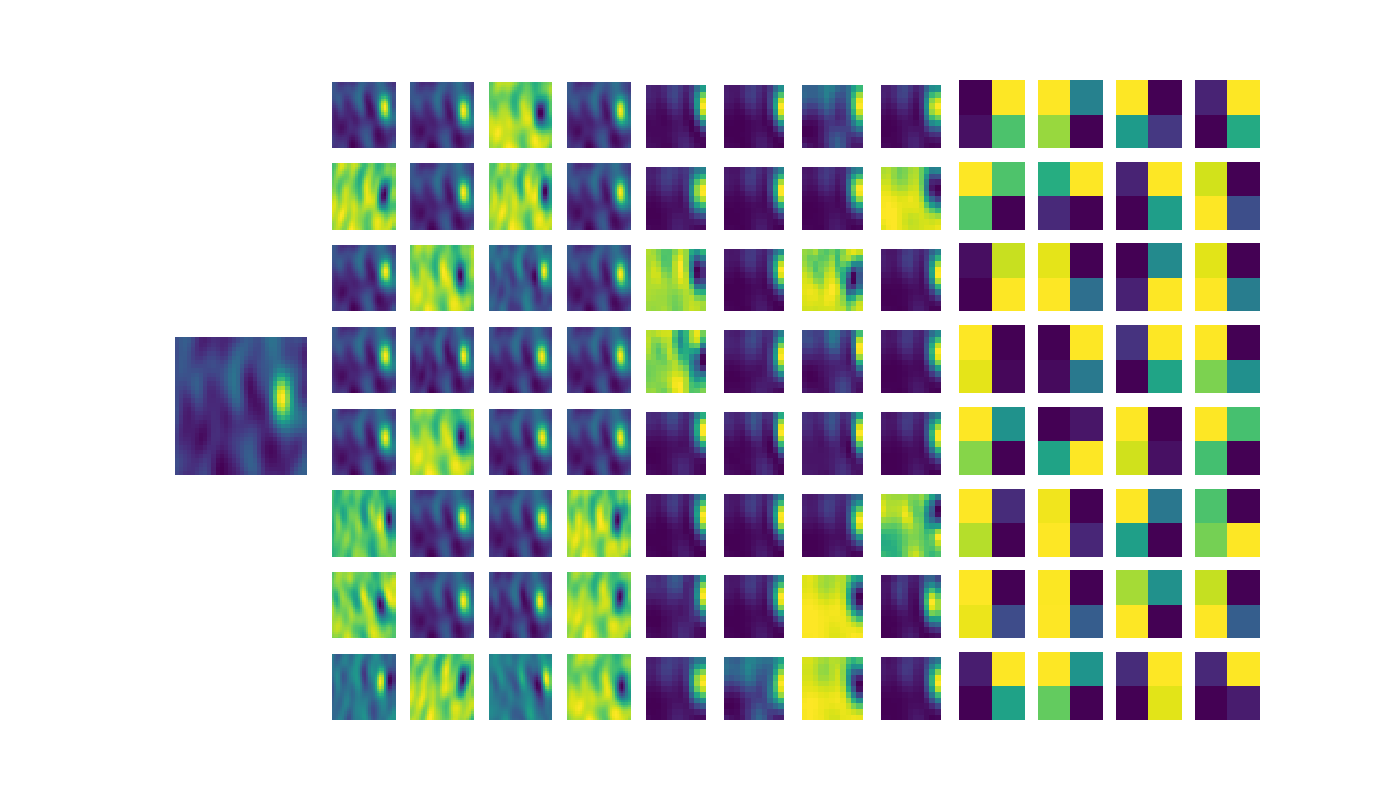
\includegraphics[width=\textwidth]{images/rgz_cnn}
        \caption{The effects of convolutional layers on an input image. The
          left-most image is the original radio image. The other images are the
          32 images output from each of the three convolutional layers.}
        \label{fig:rgz-cnn}
      \end{figure}

  \subsection{Feature Analysis}
  \label{sec:feature-analysis}

    To determine the effect of each set of features on classification
    performance, we performed a feature ablation experiment. We trained a
    logistic regression classifier on the \citeauthor{norris06} label set, each
    time using a different subset of features. The lower the resulting balanced
    accuracy, the more important the held out features. This was repeated ten
    times with different $50\%$ subsets of the training set. When holding out
    the WISE magnitude features, we also held out the CNN features, since we
    found that the CNN features tended to dominate results. These results are
    plotted in Figure \ref{fig:feature-ablation} and the means and standard
    deviations of the balanced accuracies are tabled in Table
    \ref{tab:feature-ablation}.

    \begin{figure}[!ht]
      \centering
      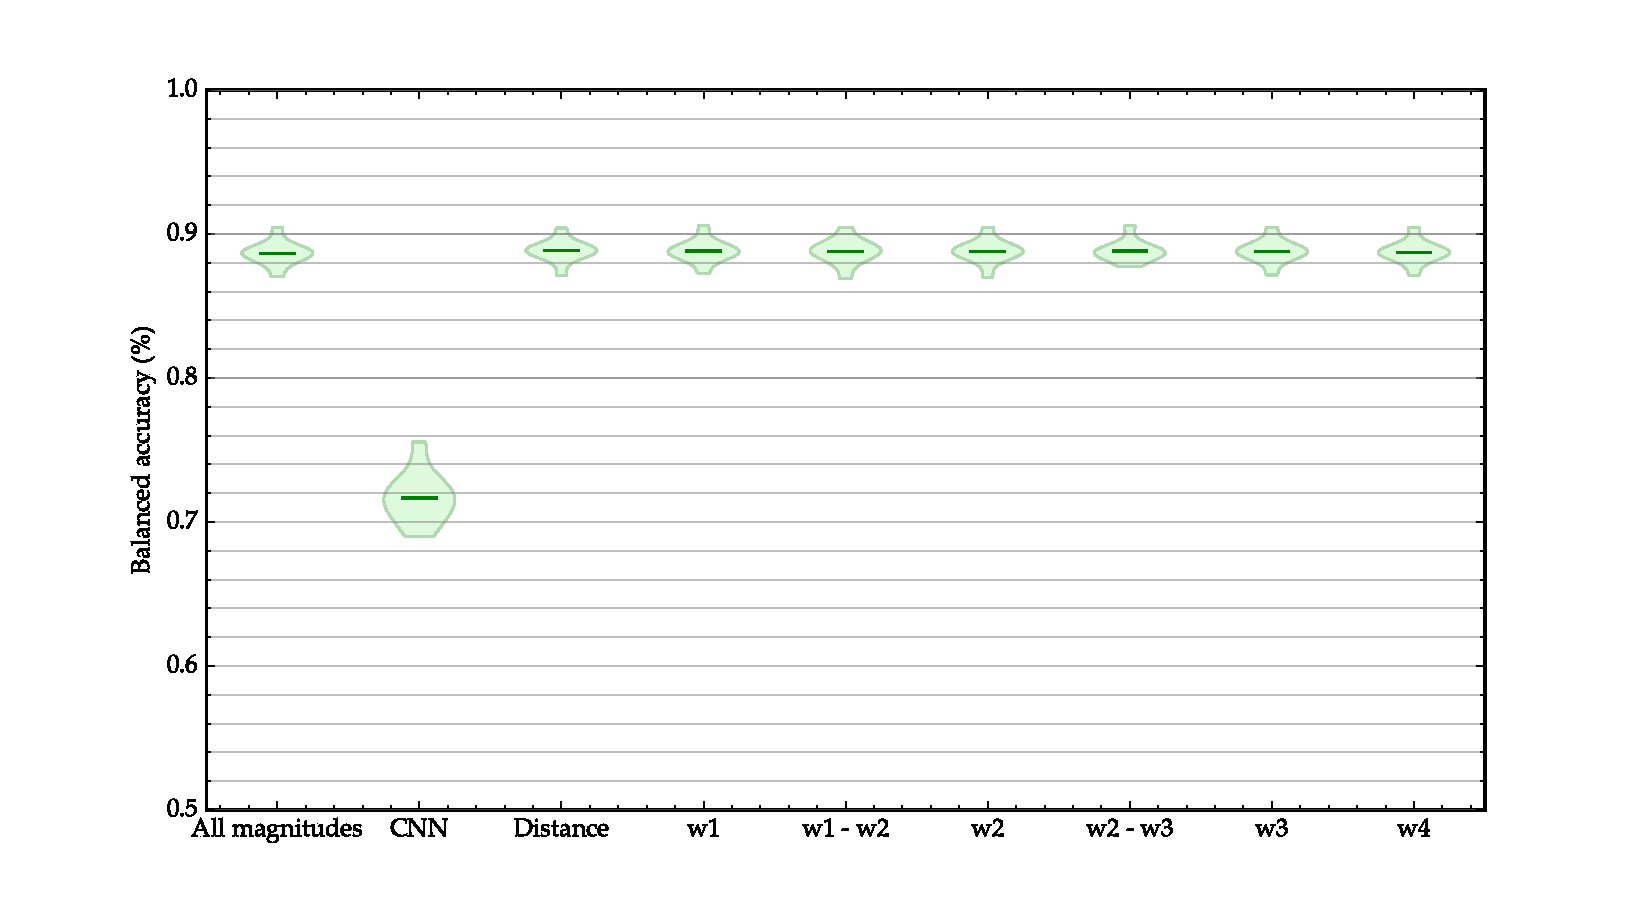
\includegraphics[width=\textwidth]{%
        images/experiments/feature_ablation.pdf}
      \caption{Balanced accuracy of logistic regression trained on the
        \citeauthor{norris06} label set with different subsets of features. The
        horizontal axis indicates which features were used for the results in
        that column.}
      \label{fig:feature-ablation}
    \end{figure}

    \begin{table}[!ht]
      \centering
      \begin{tabular}{r|c}
        \textbf{Features} & \textbf{Mean Balanced Accuracy}\\\hline
        No distance & $(88.82 \pm 0.70)\%$\\
        All features & $(88.74 \pm 0.78)\%$\\
        No magnitudes & $(88.73 \pm 0.83)\%$\\
        CNN only & $(88.66 \pm 0.81)\%$\\
        No CNN + no $w1 - w2$ & $(81.32 \pm 0.81)\%$\\
        Distance only & $(79.01 \pm 0.58)\%$\\
        No CNN & $(71.67 \pm 1.71)\%$\\
        No CNN + no $w1$ & $(71.67 \pm 1.71)\%$\\
        No CNN + no $w2$ & $(71.67 \pm 1.71)\%$\\
        No CNN + no $w3$ & $(71.67 \pm 1.71)\%$\\
        No CNN + no $w4$ & $(71.67 \pm 1.70)\%$\\
        No CNN + no $w2 - w3$ & $(71.15 \pm 2.16)\%$\\
        Magnitudes only & $(56.47 \pm 0.70)\%$\\
      \end{tabular}
      \caption{Balanced accuracy of logistic regression trained on the
        \citeauthor{norris06} label set with different subsets of features. The
        rows are sorted from highest accuracy to lower.}
      \label{tab:feature-ablation}
    \end{table}

\section{Choosing a Binary Classifier}
\label{sec:binary-classifiers}
  
  \begin{figure}[!ht]
    \centering
    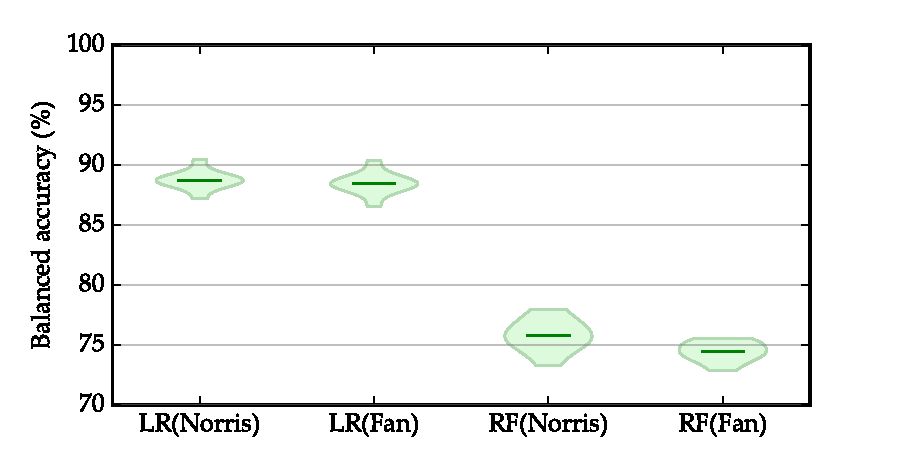
\includegraphics[width=\textwidth]{images/experiments/lr_rf}
    \caption{Comparison of logistic regression and random forests on the galaxy
      classification task, trained on the \citet{norris06} and \citet{fan15}
      label sets, and tested against the \citet{norris06} label set.}
  \end{figure}

  To compare the performance of logistic regression with random forests on the
  galaxy classification task, I performed the following experiment. First, I
  generated five test sets of WISE objects. Then, using all other WISE objects
  as a training set, I trained a logistic regression classifier for each test
  set, first using labels from \citet{norris06}, and then, separately, using
  labels from \citet{fan15}. I then computed the balanced accuracy for each
  classifier. Finally, I repeated the experiment for random forests.

  \begin{itemize}
    \item LR used L2 regularisation with C = 1 strength
    \item RF used sqrt(features)
  \end{itemize}

  To generate the test sets, I first selected at random half of all ATLAS
  objects. I then added all WISE objects within $1'$ of a selected ATLAS object
  to the test set. This was repeated for each test set. The motivation for first
  selecting ATLAS objects rather than drawing WISE objects directly is that WISE
  objects have overlapping features since radio features are taken from a patch
  of sky centred on each object, and WISE objects tend to be close together.
  Objects from the test sets were then removed at random until all test sets
  were the same size. Each test set contained $13605$ WISE objects.
  \todo{Check numbers.}

\section{Handling Crowd Labels}
\label{sec:rgz-crowd-labels}

  While we want to train a classifier on the crowdsourced labels from the Radio
  Galaxy Zoo, it is unclear how we should aggregate the labels. Some methods for
  aggregation are described in Section \ref{sec:crowd-labels}. Which method will
  perform best on a dataset is dependent on the dataset itself, so we tested
  both variants of the \citeauthor{raykar10} algorithm and majority vote on the
  galaxy classification task.

  One key problem with the use of the \citeauthor{raykar10} algorithm is that it
  is very slow with large numbers of labellers. To help mitigate this problem,
  we tested the algorithm on a subset of labellers, chosen by three different
  measures: the 10 labellers with the most labels, the 10 labellers with the
  highest balanced accuracy assessed against the \citeauthor{norris06} labels,
  and the 10 labellers with the highest balanced accuracy assessed against the
  majority vote of all labellers. While in practice on datasets such as EMU or
  FIRST there would be no equivalent to the \citeauthor{norris06} labels, we can
  treat this test as a ``best-case'' method. For each subset of labellers, the
  \citeauthor{raykar10} algorithm was tested against logistic regression trained
  on the majority vote of just these labellers. The results are shown in Figure
  \ref{fig:rgz-raykar}.

  \begin{figure}[!ht]
    \centering
    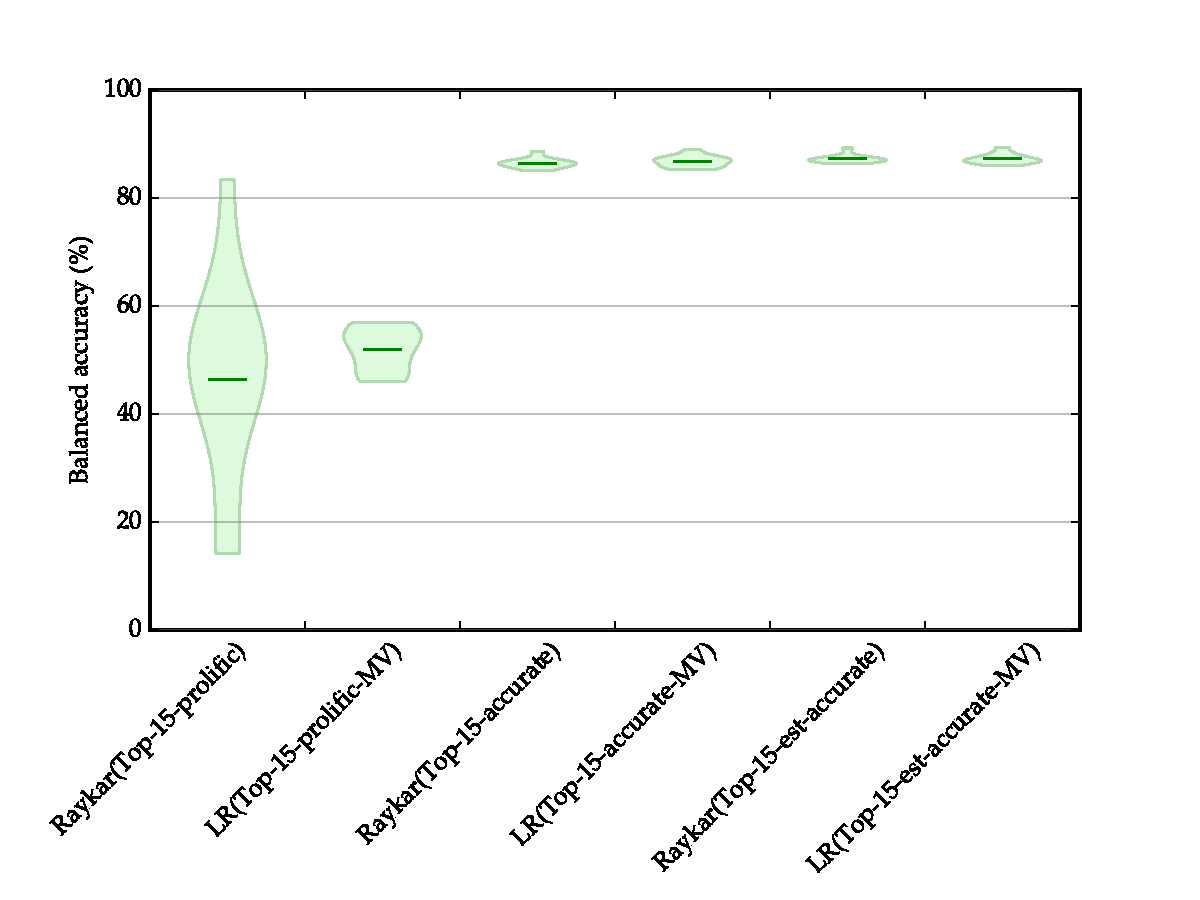
\includegraphics[width=\textwidth]{images/experiments/rgz_raykar}
    \caption{Comparison of logistic regression and \citeauthor{raykar10} on the
      galaxy classification task with different numbers of labellers.}
    \label{fig:rgz-raykar}
  \end{figure}

\section{Results}
\label{sec:rgz-results}
  
  \subsection{Classifying Galaxies}

    \todo{Make this writing considerably less terrible.}

    The infrared objects were partitioned into a testing set and a training set
    as follows. First, the radio objects were partitioned into a radio testing
    set and a radio training set, with the radio testing set containing $452$
    objects and the radio training set containing $1811$ objects. Infrared
    objects were then added to the infrared testing set if they were within $1'$
    of a radio object in the radio testing set, and added to the infrared
    training set otherwise. This was done because infrared objects that were
    close together had overlapping radio features, and thus random partitioning
    would result in the training set containing many of the features found in
    the testing set. The partitioning resulted in $5922$ objects in the testing
    set and $18218$ objects in the training set.

    For each infrared object, features and labels were generated as described in
    Sections \ref{sec:features} and \ref{sec:consensuses}, respectively. Note
    that the labels were sourced from the Radio Galaxy Zoo. A logistic
    regression classifier was then trained on the training set using binary
    cross-entropy loss, with loss of each data point weighted based on the
    frequency of its label.

    The classifier was then used to classify the objects in the testing set. The
    labels were compared to those found by \citet{norris06} as described in
    Section \ref{sec:norris}, resulting in $80.14\%$ balanced accuracy.
    \todo{This number is out of date.}

    \todo{ROC/precision--recall curves}

    \begin{figure}[!ht]
      \centering
      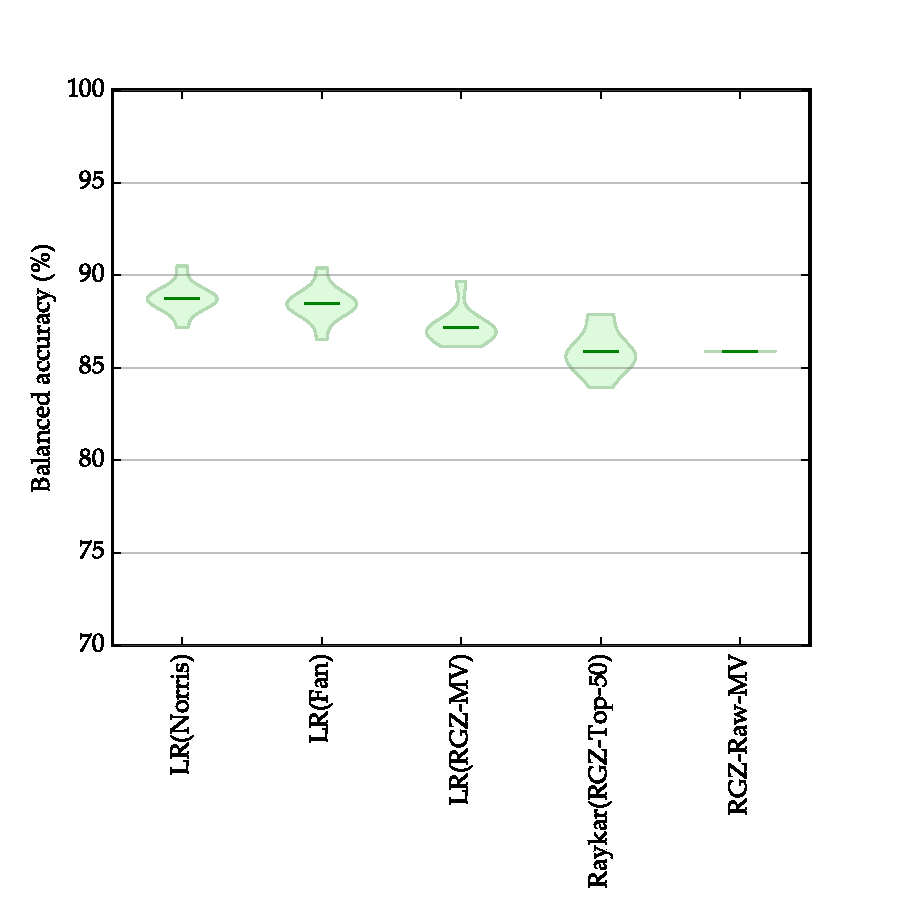
\includegraphics[width=\textwidth]{images/experiments/predictors.pdf}
      \caption{Performance of logistic regression on the galaxy classification
        task, trained on different sets of labels and tested on the galaxies
        where \citeauthor{norris06} and \citeauthor{fan15} labels agree. LR($Y$)
        indicates logistic regression trained on $Y$. RGZ-MV is the set of
        majority vote labels from the Radio Galaxy Zoo. RGZ-Raw-MV is the
        majority vote of all crowd labels and is included for comparison.}
    \end{figure}

  \subsection{Number of Training Examples}

    \begin{figure}[!ht]
      \centering
      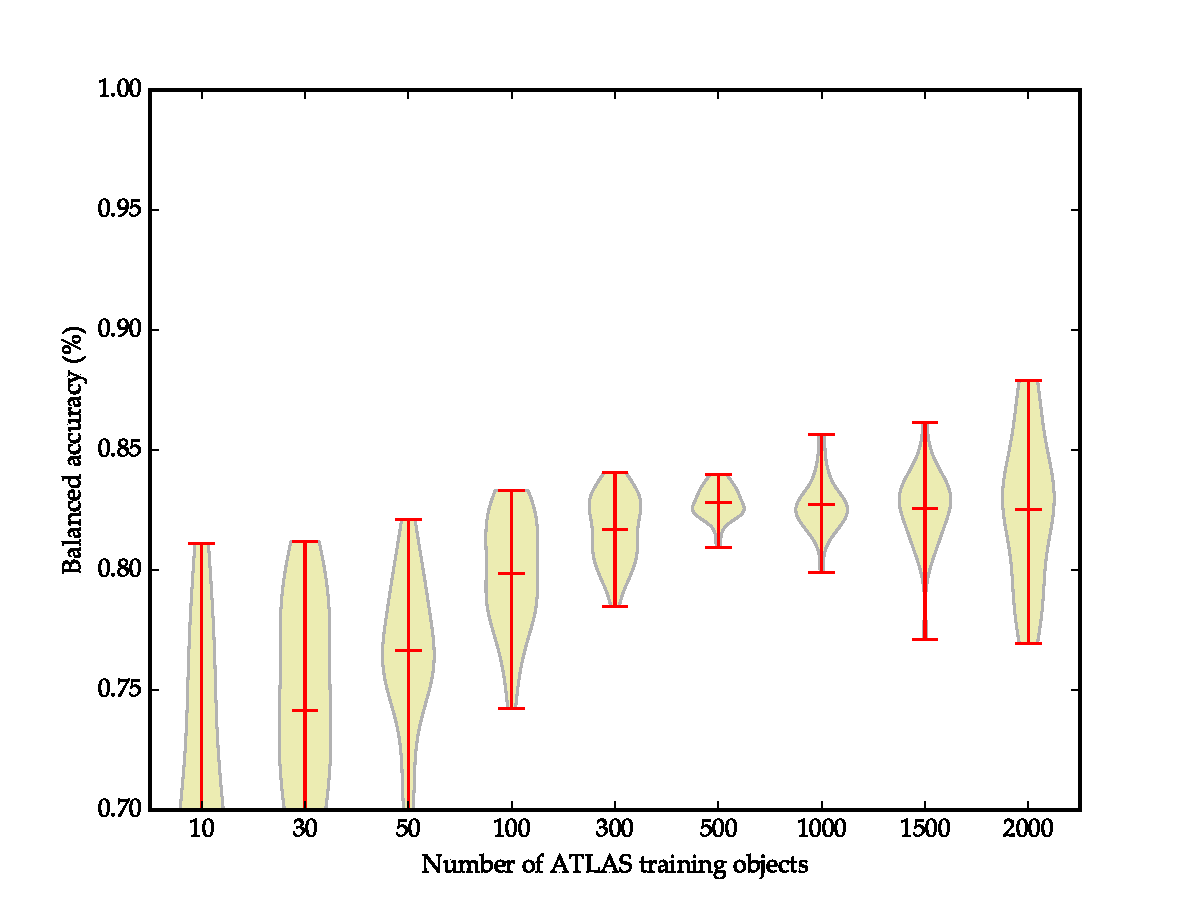
\includegraphics[width=\textwidth]{images/experiments/passive.pdf}
      \caption{Performance of logistic regression on the galaxy classification
        task, trained on different amounts of the \citeauthor{norris06} label
        set.}
    \end{figure}

  \todo{Discuss results}